\documentclass{beamer}
\usepackage{minted}
\setbeamertemplate{caption}{\raggedright\insertcaption\par}
\newcommand\Fontvi{\fontsize{9.5}{7.2}\selectfont}
\usepackage[T1]{fontenc}
\begin{document}

\title{Analisi della sicurezza binaria di WebAssembly}
\author{Alessandro Arata}
\institute{Universitá di Genova}
\date{\today}

\begin{frame}
  \titlepage
\end{frame}

\begin{frame}
  \frametitle{WebAssembly}
  \begin{columns}
    \begin{column}{0.6\textwidth}
      \begin{itemize}
        \item è un linguaggio bytecode che offre tempi di esecuzione rapidi e un
        formato portabile e compatto
        \item è stato ideato come un \textbf{target di compilazione}
        \begin{itemize}
          \item esistono compilatori da C(++), Rust ed altri linguaggi
        \end{itemize}
        \item è pensato per eseguire codice in maniera efficiente sui
          \textbf{browser} 
        \begin{itemize}
          \item può essere eseguito anche in ambienti di backend come Node.js
        \end{itemize}
      \end{itemize}
    \end{column}
    \begin{column}{0.4\textwidth}
      \centerline{
\includegraphics[width=3cm,height=3cm,keepaspectratio]{images/logo.png}}
      \newline\newline\newline
      \centerline{
\includegraphics[width=4cm,height=4cm,keepaspectratio]{images/browser-logos.png}}
    \end{column}
  \end{columns}
\end{frame}

\begin{frame}
  \frametitle{WebAssembly - gestione della memoria}
  \begin{columns}
    \begin{column}{0.6\textwidth}
  \begin{itemize}
    \item staticamente tipato con quattro tipi primitivi: \textbf{i32/64},
      \textbf{f32/64}
      \item lo stack delle chiamate e le variabili primitive sono gestiti dalla macchina virtuale
    \item i tipi non primitivi (stringhe, indirizzi, classi, struct...) vengono
      salvati nella \textbf{memoria lineare}
    \item la memoria lineare è gestita dal programma
  \end{itemize} 
  \end{column}
    \begin{column}{0.4\textwidth}
  \centerline{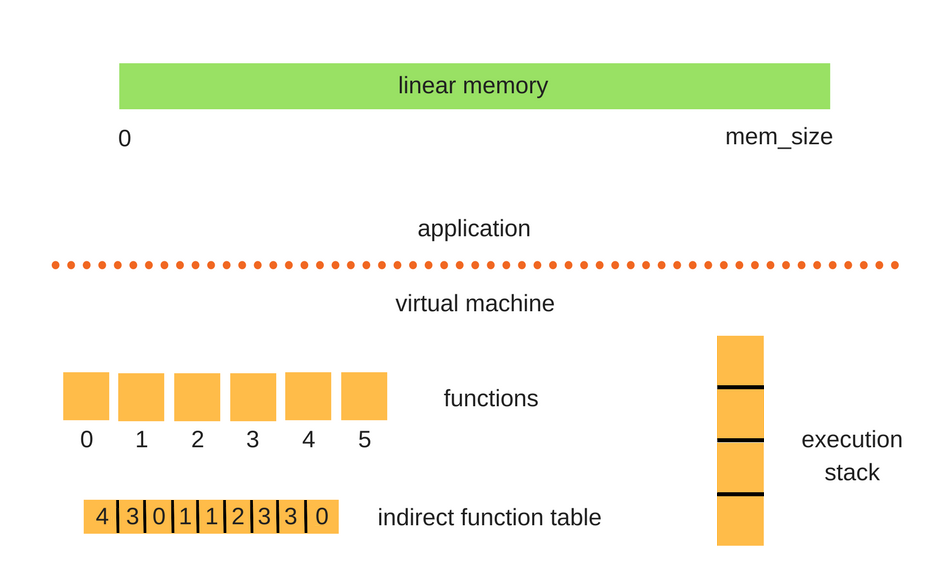
\includegraphics[width=10cm,height=3.5cm,keepaspectratio]{images/linmem.png}}
    \end{column}
  \end{columns}
\end{frame}

\begin{frame}[fragile]
  \frametitle{hello-world.wat}
  \Fontvi
  \begin{minted}{c}
    puts("Hello, world!");
  \end{minted}

  \vspace{0.2in}
  \centerline{corrisponde nel formato assembly di WebAssembly  (\textbf{.wat}) a}
  \vspace{0.2in}

  \begin{minted}{wat}
    (module
      ;; Imports from JavaScript namespace and log function
      (import  "console"  "log" (func  $log (param  i32  i32)))
      ;; Import 1 page of memory
      (import  "js"  "mem" (memory  1))
      ;; Data section of our module
      (data (i32.const 0) "Hello, world!")
      ;; Function declaration: Exported as helloWorld(), no arguments
      (func (export  "helloWorld")
        ;; pass offset 0 to log
        i32.const 0
        ;; pass length 13 to log (strlen of sample text)
        i32.const 13          
        call  $log
      )
    ) 
  \end{minted}
\end{frame}

\begin{frame}
  \frametitle{Memoria lineare}
  \begin{columns}
    \begin{column}{0.6\textwidth}
      \begin{itemize}
        \item array \textbf{globale} di byte indirizzato da puntatori di tipo i32
      \item è divisa in \textbf{regioni} per heap, stack e dati statici
        \item contiene tipi non primitivi 
        \item è sia leggibile che scrivibile ma non eseguibile 
        \item tutta la memoria risulta allocata al programmatore: ogni puntatore compreso tra [0, mem\_max] è valido 
      \end{itemize}
    \end{column}
    \begin{column}{0.4\textwidth}
      \centerline{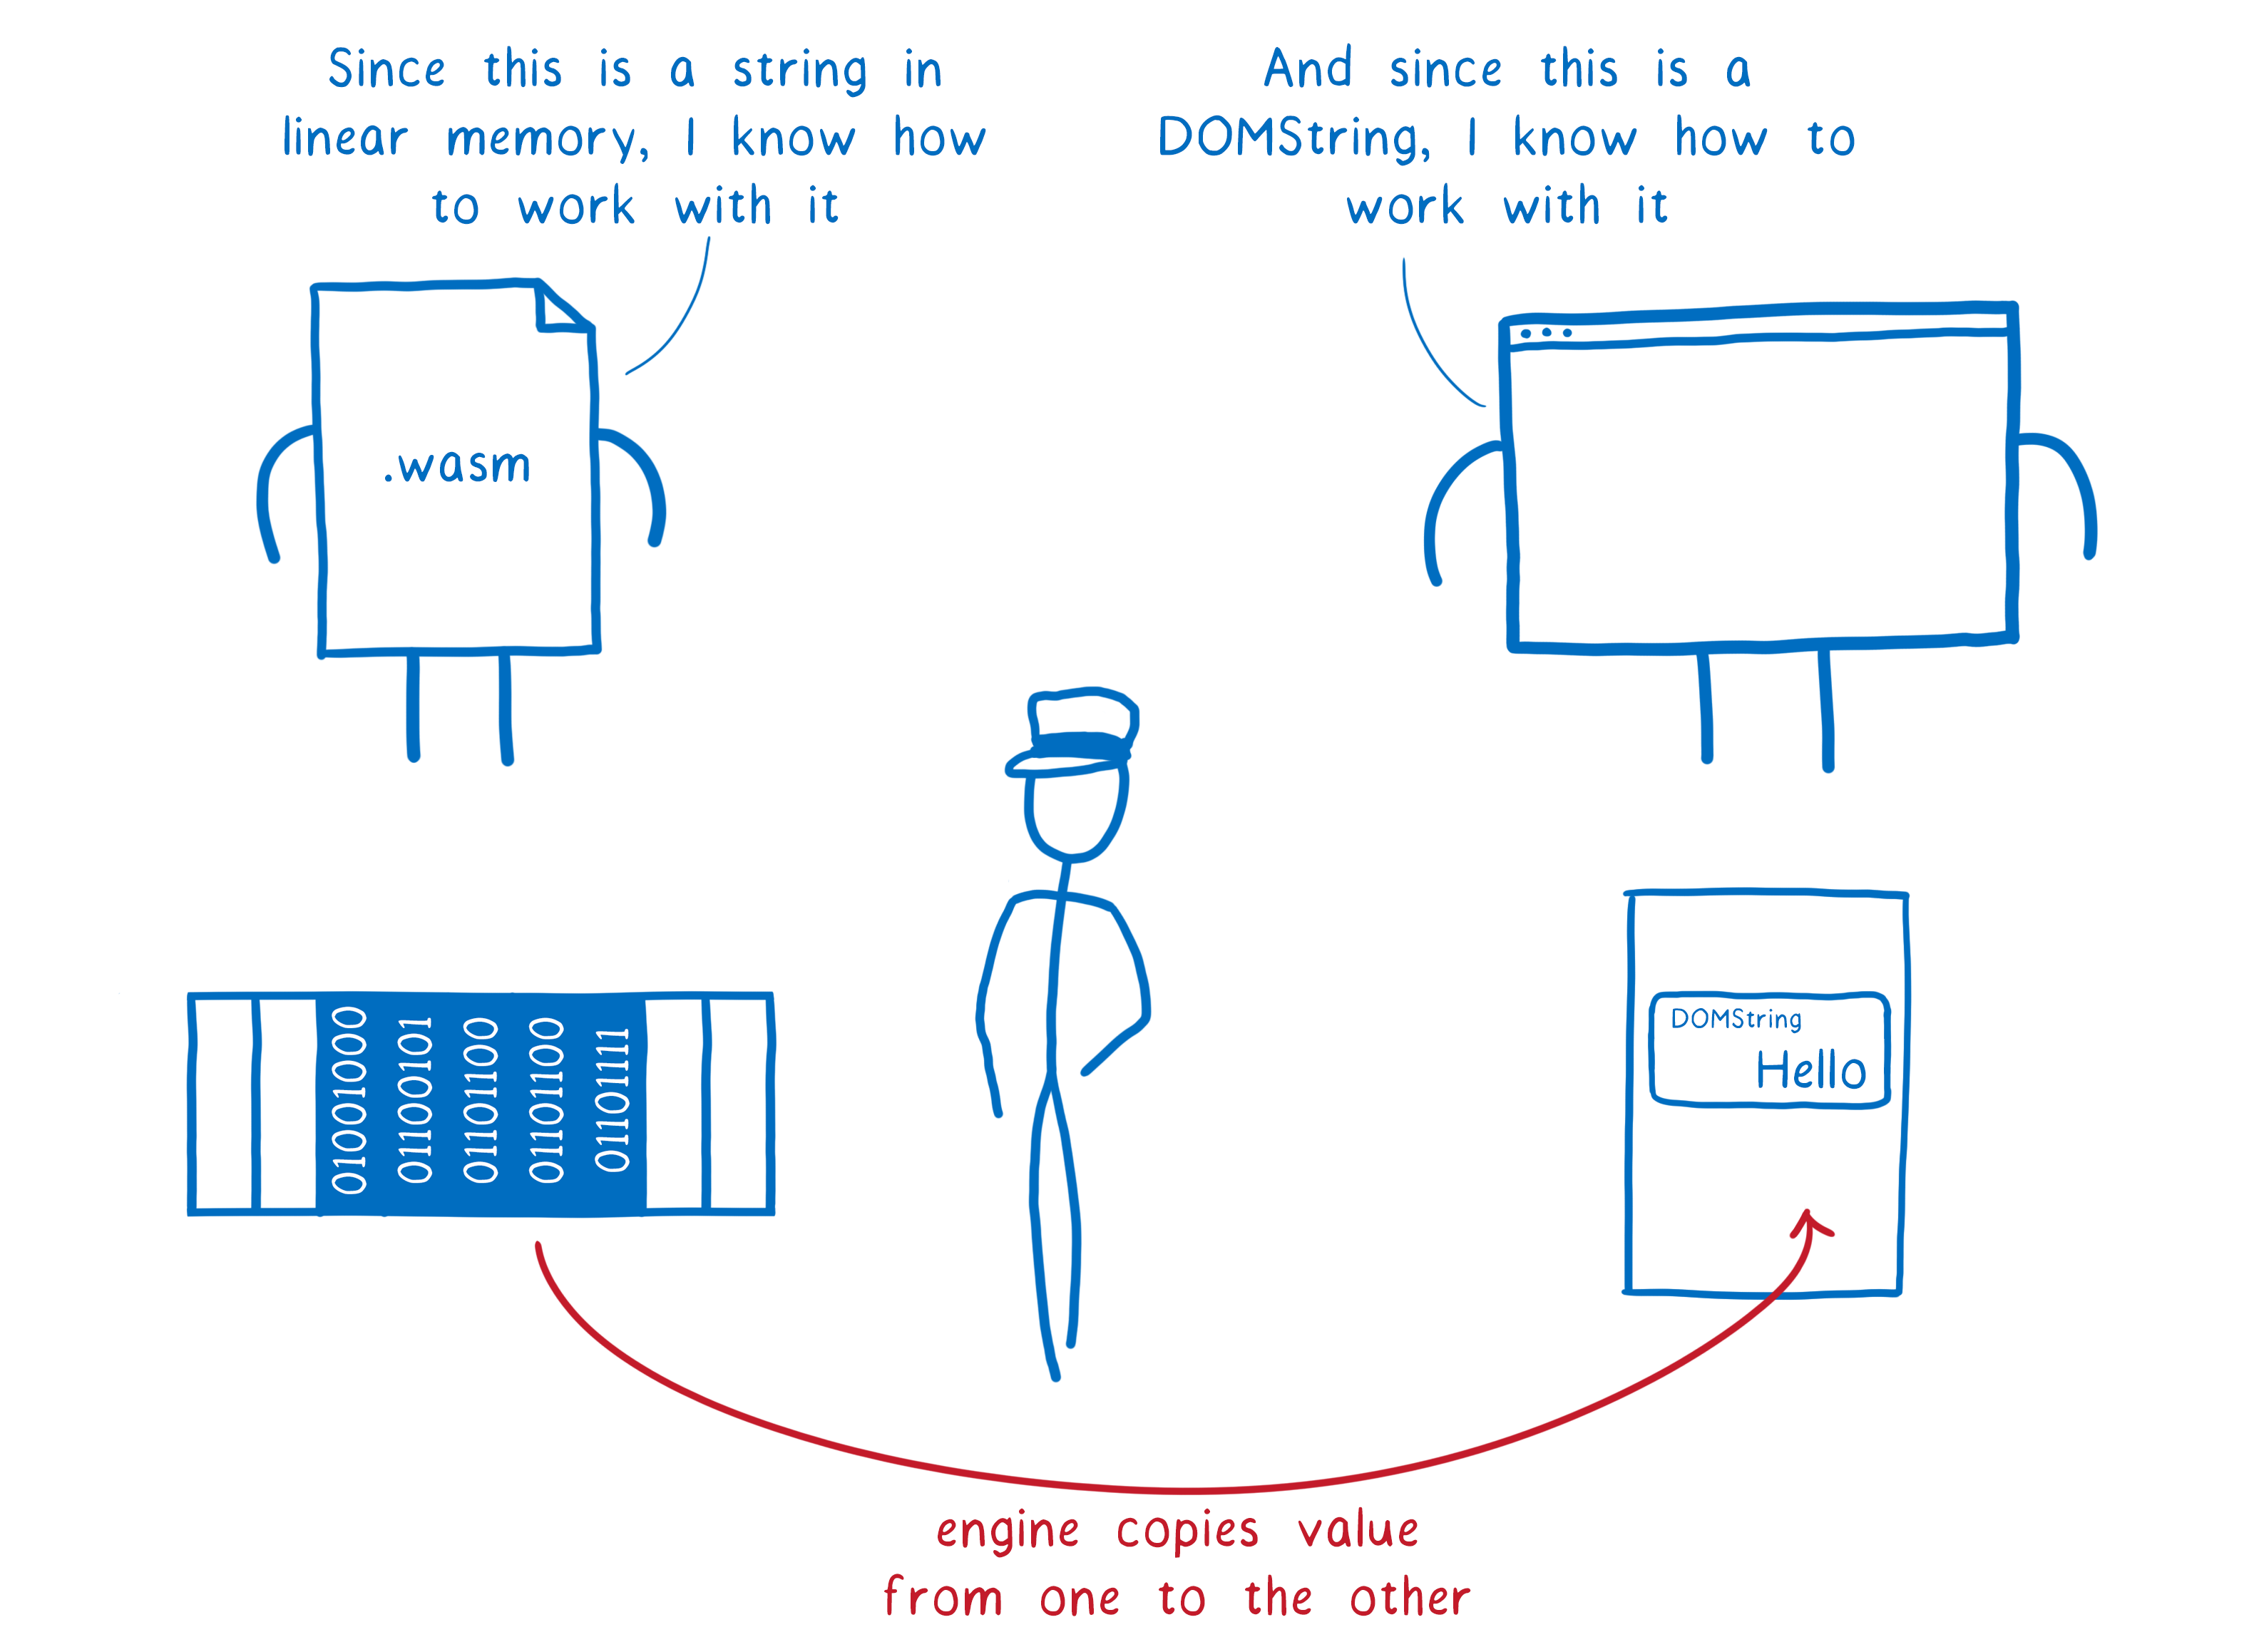
\includegraphics[width=8cm,height=4cm,keepaspectratio]{images/memman.png}}
    \end{column}
  \end{columns}
\end{frame}

\begin{frame}
  \frametitle{Principali mitigazioni nei binari nativi}
  \begin{itemize}
    \item i binari nativi offrono diverse mitigazioni in maniera da rendere
      difficile l'utilizzo di exploit della memoria
      \begin{itemize}
        \item \textbf{Address Layout Space Randomization} (ASLR)      
        \item \textbf{Guard page}        
        \item \textbf{Stack canary} 
      \end{itemize}
    \item esistono sezioni non scrivibili per i dati costanti in modo che
      non possano essere sovrascritti
    \item la memoria del processo è divisa in pagine non necessariamente sempre
      mappate
      \begin{itemize}
        \item un attaccante deve evitare di accedere a pagine non allocate
          (verrebbe sollevato un fault)
      \end{itemize}
  \end{itemize}
\end{frame}

\begin{frame}
  \frametitle{Memoria lineare - sicurezza binaria}
  \begin{columns}
    \begin{column}{0.6\textwidth}
      \begin{itemize}
        \item no \textbf{ASLR}: la posizione di una elemento è "predicibile"
        \item nessuna \textbf{guard page} tra le regioni: è possibile
          sovrascrivere dati di regioni contigue
        \item nessuna \textbf{stack canary}: il binario non controlla da sè se si scriva
          oltre lo spazio
          allocato per il buffer
        \item ogni area è scrivibile: dati apparentemente costanti possono essere
          sovrascritti
        \item per l'attaccante ogni puntatore è valido dato che non esistono page fault
      \end{itemize}
    \end{column}
    \begin{column}{0.4\textwidth}
      \centerline{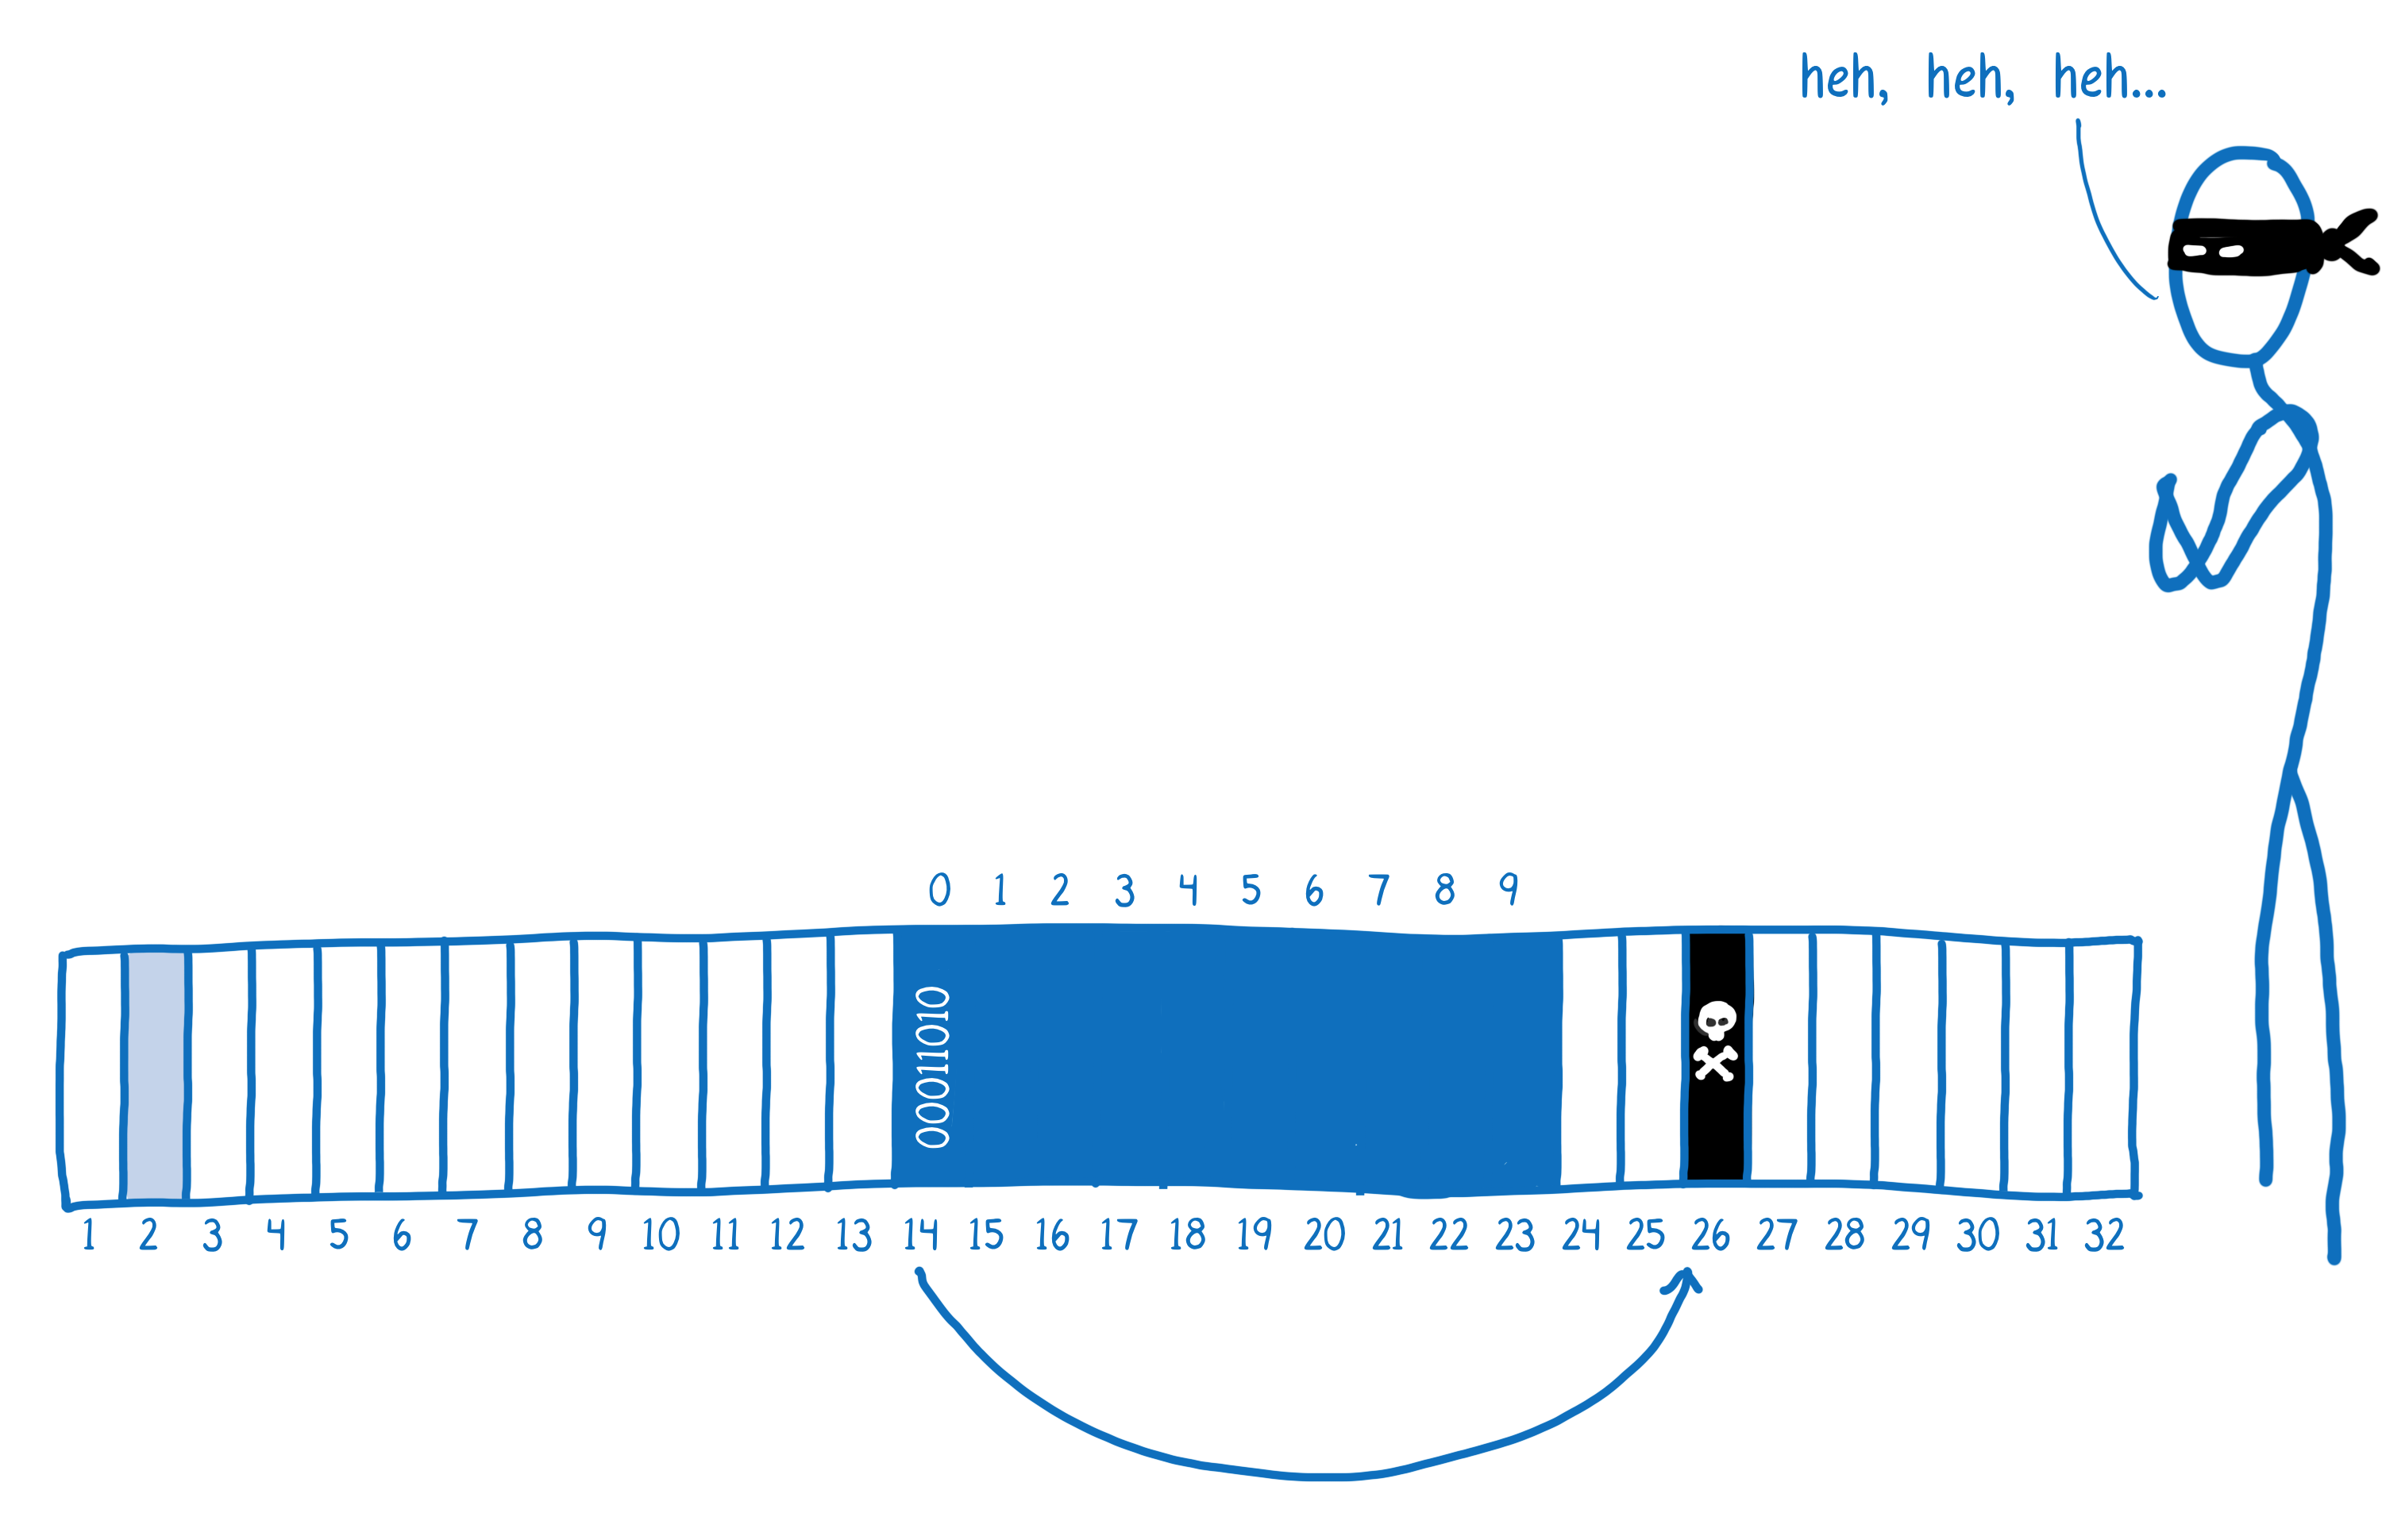
\includegraphics[width=5cm,height=3cm,keepaspectratio]{images/attack.png}}
    \end{column}
  \end{columns}
\end{frame}

\begin{frame}[fragile]
  Rispetto alle mitigazioni include nei binari nativi, la memoria lineare di
  WebAssembly non offre molto dal punto di vista della sicurezza binaria.
\newline\newline
  Cosa succede se si compila un programma \textbf{vulnerabile} in WebAssembly?
\newline\newline
  \begin{minted}{c}
    void vuln() {
      char buffer[16];
      gets(buffer); // !!!
    }
  \end{minted}
\end{frame}

\begin{frame}
  \frametitle{Primitiva di attacco: buffer overflow}
  \begin{columns}
    \begin{column}{0.6\textwidth}
      \begin{itemize}
        \item se la lunghezza dell'input dell'utente non viene controllata,
          è possibile scrivere al di fuori di un buffer
        \begin{itemize}
          \item si possono sovrascrivere variabili locali o indirizzi di
            ritorno
        \end{itemize}
        \item funzioni come \textbf{gets()} e \textbf{strcpy()} permettono questo tipo di attacco  
      \end{itemize} 
    \end{column}
    \begin{column}{0.4\textwidth}
      \centerline{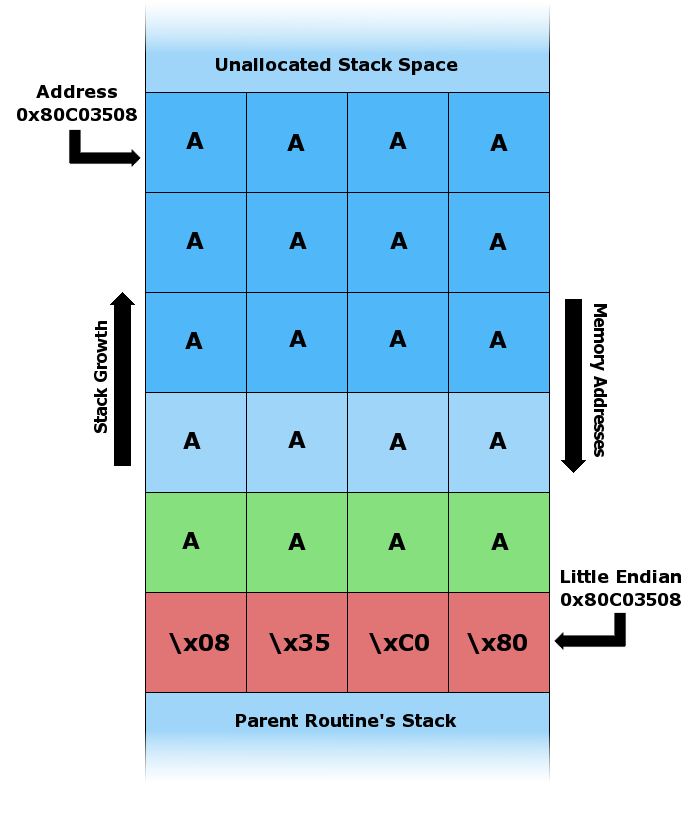
\includegraphics[width=10cm,height=6.5cm,keepaspectratio]{images/stack.png}}
    \end{column}
  \end{columns}
\end{frame}

\begin{frame}[fragile]
  \frametitle{Sovrascrivere dati "costanti"}
  \Fontvi
  \begin{minted}{c}
    char *other_data = "AAAA";

    static char *safe_script = 
      "console.log('this should be safe, shouldn\\'t it?')";


    int main() {
       
      emscripten_run_script(safe_script);
    
    }


    void vuln(const char* input) {
    
      strcpy(other_data, input);

    }
  \end{minted}
\end{frame}

\begin{frame}
  \frametitle{Sovrascrivere dati "costanti"}
  \begin{columns}
    \begin{column}{0.55\textwidth}
      \begin{itemize}
        \item le variabili statiche sono salvate nella regione \textbf{data}
          (scrivibile)
        \item \textbf{strcpy()} non effettua controlli sulla dimensioni dell'input: è possibile sovrascrivere dati sullo stack
        \begin{itemize}
          \item un overflow nello stack riesce a scrivere nella regione \textbf{data}
        \end{itemize}
      \item sovrascrivendo la stringa contenuta nella variabile
        \textbf{safe\_script} si
          possono eseguire comandi JavaScript arbitrari
        \begin{itemize}
          \item \textbf{XSS} nel browser
          \item \textbf{RCE} con Node.js
        \end{itemize}

            \end{itemize}
    \end{column}
    \begin{column}{0.45\textwidth}
      \begin{figure}[htbp]
        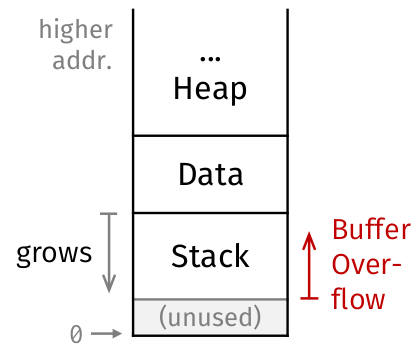
\includegraphics[width=4cm,height=6cm,keepaspectratio]{images/memory_layout.png}
        \newline\newline\newline
        \begin{figure}
          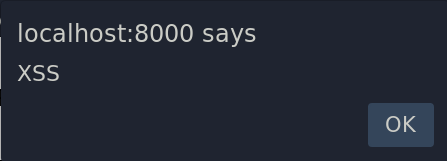
\includegraphics[width=4cm,height=6cm,keepaspectratio]{images/xss.png}
          \caption{Chiamando \textbf{vuln()} con la stringa
          ";;;;;;;;;;;;;;;;;;;;;;;;;;;;;;;;;alert('XSS')"}
        \end{figure}
        \end{figure}
    \end{column}
  \end{columns}
\end{frame}

\begin{frame}[fragile]
  \frametitle{Sovrascrivere dati sullo heap}
  \begin{itemize}
    \item similmente è possibile sovrascrivere dati sullo heap
    \item la libreria \textbf{libpng} contiene un buffer overflow che
      è possibile sfruttrare convertendo un immagine da pnm a png 
  \end{itemize}
  \begin{minted}{c++}
    int main() {
      std::string img_tag = 
        "<img src='data:image/png;base64,";
      // CVE-2018-14550
      pnm2png("input.pnm", "output.png");        
      img_tag += file_to_base64("output.png") + "'>";
      emcc::global("document").call("write", img_tag);
    }
  \end{minted}
  \begin{itemize}
    \item se l'input dell'utente non viene controllato/sanitizzato, è possibile
      sovrascrivere la string \textbf{img\_tag} situata nello heap 
    \item questo causa un attacco di tipo XSS nel browser
  \end{itemize}
\end{frame}

\begin{frame}
  \frametitle{Sovrascrivere dati sullo heap}
  \Fontvi 
  \begin{columns}
    \begin{column}{0.5\textwidth}
      \begin{figure}
        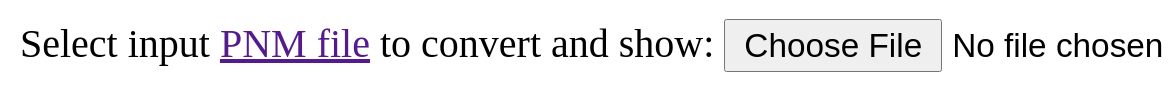
\includegraphics[width=5cm,height=6cm,keepaspectratio]{images/site.png}
        \caption{Il sito chiede all'utente un'immagine in input: non vengono
        fatti controlli sul tipo di file} 
      \end{figure} 
      \begin{figure}
        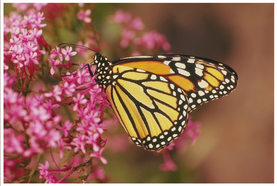
\includegraphics[width=4cm,height=4cm,keepaspectratio]{images/butfly.png}
        \caption{Se l'utente immette un'immagine, questa viene convertita
        e mostrata nel browser} 
      \end{figure} 

    \end{column}
    \begin{column}{0.5\textwidth}
      Utilizzando come payload
      \newline\newline\newline
      AAAAAAAAAAAAAAAAAAAAAAAA...
      <script>alert('XSS')</script><!- -
      \newline\newline\newline
      si effettua un overflow nello stack che permette di sostituire al tag
      \textbf{<img>} il tag \textbf{<script>} nello heap: questo provoca un attacco di
      tipo XSS
      \newline\newline\newline
      \centerline{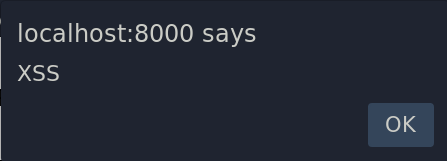
\includegraphics[width=5.5cm,height=5.5cm,keepaspectratio]{images/xss.png}}
    \end{column}

  \end{columns}
\end{frame}


\begin{frame}
  \frametitle{Conclusioni}
  \begin{itemize}
    \item WebAssembly ha reintrodotto vulnerabilitá precendentemente mitigate
      e introdotto nuovi tipi di attacchi, come sovrascivere dati costanti
    \item  
  \end{itemize}
\end{frame}

\begin{frame}
  \frametitle{Bibliografia}
  \begin{enumerate}
    \item Daniel Lehmann, Johannes Kinder, Michael Pradel: \emph{"Everything Old is New Again:
      Binary Security of WebAssembly"}
    \item Brian McFadden, Tyler Lukasiewicz, Jeff Dileo, Justin Engler:
      \emph{"Security Chasms of WASM"}
  \end{enumerate}
\end{frame}

\end{document}
